\pgfdeclarelayer{backwrapping}
\pgfdeclarelayer{frontwrapping}
\pgfsetlayers{backwrapping,main,frontwrapping}

\tikzset{
    wrapping/.style={
        draw=black!80, 
        line cap=round, 
        line join=round, 
        ultra thick},
    nucleosome/.style={
        fill=red!40, 
        fill opacity=.9, 
        draw=none},
    top cylinder/.style={
        fill=red!60, 
        fill opacity=.9
    }
}


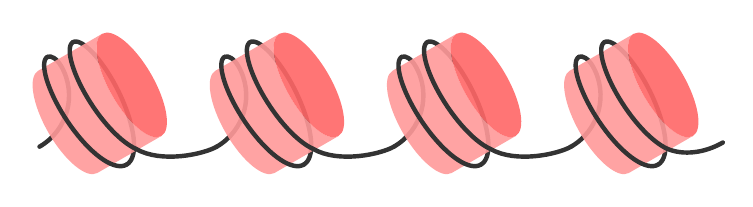
\begin{tikzpicture}[scale=0.75]

\foreach \q [remember=\q as \p] in {1, 2, 3, 4}{

\begin{scope}[shift={(\q*3,0)}, rotate=30]
\path [nucleosome] 
    (0,1) 
    arc (90:270:0.375 and 1) -- (1.25,-1) 
    arc (270:90:0.375 and 1) -- cycle;
\path [top cylinder] 
    (1.625, 0) arc (0:360:0.375 and 1) -- cycle;

\begin{scope}[shift={(0.25,0)}]
\begin{pgfonlayer}{backwrapping}
\draw [wrapping] 
    (0.25, -1.125) 
    \foreach \i in {180,185,...,360}{ -- (\i/720+0.375*sin -\i, 1.125*cos \i)};
\draw [wrapping] (0, 1.125)  arc(90:0:0.125cm and 0.25cm) arc(0:-90:1cm and 1cm) coordinate (wrapping-start-\q);
\end{pgfonlayer}

\begin{pgfonlayer}{frontwrapping}
\draw [wrapping] 
    (0, 1.125)  
    \foreach \i in {0,5,...,180}{ -- (\i/720+0.375*sin -\i,1.125*cos \i)}
    [shift={(0.5,0)}]
    (0, 1.125) 
    \foreach \i in {0,5,...,150}{ -- (\i/720+0.375*sin -\i,1.125*cos \i)} coordinate (wrapping-end-\q);
\end{pgfonlayer}
\end{scope}
\ifnum\q>1
    \draw [wrapping] (wrapping-end-\p) .. controls ++(-60:0.5cm)  and ++(180:0.25cm) .. (wrapping-start-\q);
\fi
\ifnum\q=4
\draw [wrapping] (wrapping-end-\q) arc (210:270:1cm and 0.75cm);
\fi
\end{scope}
}

\end{tikzpicture}